\documentclass[numbers=noenddot,12pt,a4paper]{scrartcl}
\usepackage[greek,ngerman]{babel}
\usepackage[T1]{fontenc}
\usepackage[utf8]{inputenc}
\usepackage{fullpage}
\usepackage{libertine}
\usepackage{ziffer}
\usepackage{graphicx}
\usepackage{units}
\usepackage[infoshow]{tabularx}
\usepackage{amsmath}
\usepackage{amssymb}
\usepackage{wrapfig}
\usepackage{esint}
\usepackage{float}
\usepackage{wrapfig}
\usepackage[font=small]{caption}
\usepackage{subcaption}
\usepackage{lscape}
\usepackage{hyperref}

\renewcommand{\thefigure}{Abb. \arabic{figure}}

\captionsetup[wrapfigure]{name=}
\captionsetup[figure]{name=}
\newcommand{\degree}{^\circ}
\newcommand{\diff}{\textnormal{d}}
\newcommand{\tenpo}[1]{\cdot 10^{#1}}
\newcommand{\greek}[1]{\greektext#1\latintext}
\newcommand{\ix}[1]{_\text{#1}}
\newcommand{\imag}{\mathbf{i}}
\newcommand{\signum}{\text{sgn}}

\title{Protokoll: Chaos und Bifurkation am Beispiel des erregten Pendels}
\author{Tom Kranz, Philipp Hacker}
\date{\today}

\begin{document}
%\setcounter{page}{2}
%\setcounter{section}{1}
\maketitle
\begin{center}
Betreuer: T. Schumann \\
Versuchsdatum: 28.10.2014/29.10.2014 \\
\begin{table}[h]
\centering
Note: %TODO Gute Note erhalten :)
\begin{tabularx}{1.5cm}{|X|}
\hline \\ \\
\hline
\end{tabularx}
\end{table}
\end{center}
\vspace*{\fill}
\tableofcontents
\vfill
\newpage
\section{Motivation}
In diesem Versuch wird die Natur chaotischer Prozesse am Beispiel des periodisch erregten Pendels beleuchtet. Dafür werden Messmethoden und die Darstellung des Prozesses im Phasenraum erklärt. Insbesondere wird auf das Phänomen der Bifurkation, der qualitativen Änderung des Phasenraumbilds bei geringfügiger Veränderung eines Kontrollparameters, eingegangen.
\section{Grundlagen}
\subsection{Der Versuchsaufbau}\label{ch2.1}
\begin{wrapfigure}{r}{0.5\textwidth}
	\centering
	\vspace{-2em}
	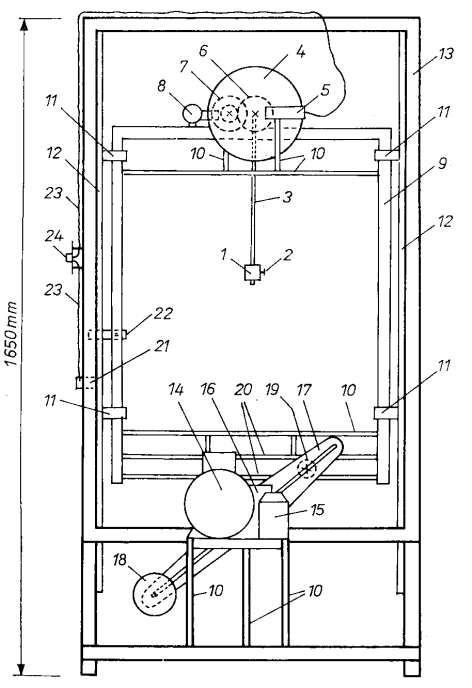
\includegraphics[width=0.5\textwidth]{pendel.png}
	\caption{Das periodisch erregte Pendel}
	\label{img:pererpen}
\end{wrapfigure}
\ref{img:pererpen} zeigt den Versuchsaufbau. Hierbei handelt es sich um ein physikalisches Pendel, dessen Hauptschwingmasse (1) über einen Stab (3) an der Drehachse ($\times$) befestigt ist. Die Masse kann durch Lösen der Stellschraube (2) auf dem Stab verschoben werden, um das Trägheitsmoment des Pendels zu beeinflussen. Zum Pendelkörper (beziehungsweise zum schwingenden Trägheitsmoment) gehören weiterhin die Winkelcodescheibe (4), die zum Auslesen der aktuellen Auslenkung mittels Auflichtschranken (5) benutzt wird und die Aluminiumscheibe der Wirbelstrombremse (7), deren 15-Zahn-Zahnrad über ein 100-Zahn-Zahnrad (6) mit der Drehachse verbunden ist. Zur Wirbelstrombremse gehört weiterhin eine magnetfeld-erzeugende Spulen-\greek{μ}-Metall-Konstruktion (8). Die Teile (9) bis (13) bilden die Halterung des Pendels, damit es sich auf und ab bewegen kann. Der Hebelarm (17) wird über ein Getriebe (16) von einem Elektromotor (14) gedreht, woraufhin sich die an den Führungsschienen (20) verschiebbar gelagerte Führungsrolle (19) im Kreis bewegt und die Halterung periodisch auf und ab beschleunigt. Über die Steuerkonsole (15) lässt sich der Elektromotor ein- und ausschalten und die Erregerfrequenz einstellen. Die Lichtschranke (21) registriert den Durchlauf des Zeigers (22) zu einer bestimmten Phasenlage der Erregung für die stroboskopische Ausgabe der Messwerte. Schließlich bildet (23) die Verkabelung und (24) ein Interface zum Abgreifen der Messwerte mittels eines Oszilloskops.\\
\subsection{Die Messung}\label{ch2.2}
Direkt gemessen wird nur die aktuelle Auslenkung des Pendels. Dies geschieht über die in \ref{img:wicosch} gezeigte Winkelcodescheibe, eine Auflichtschranke und eine Auswertungselektronik.
\begin{figure}[H]
	\centering
	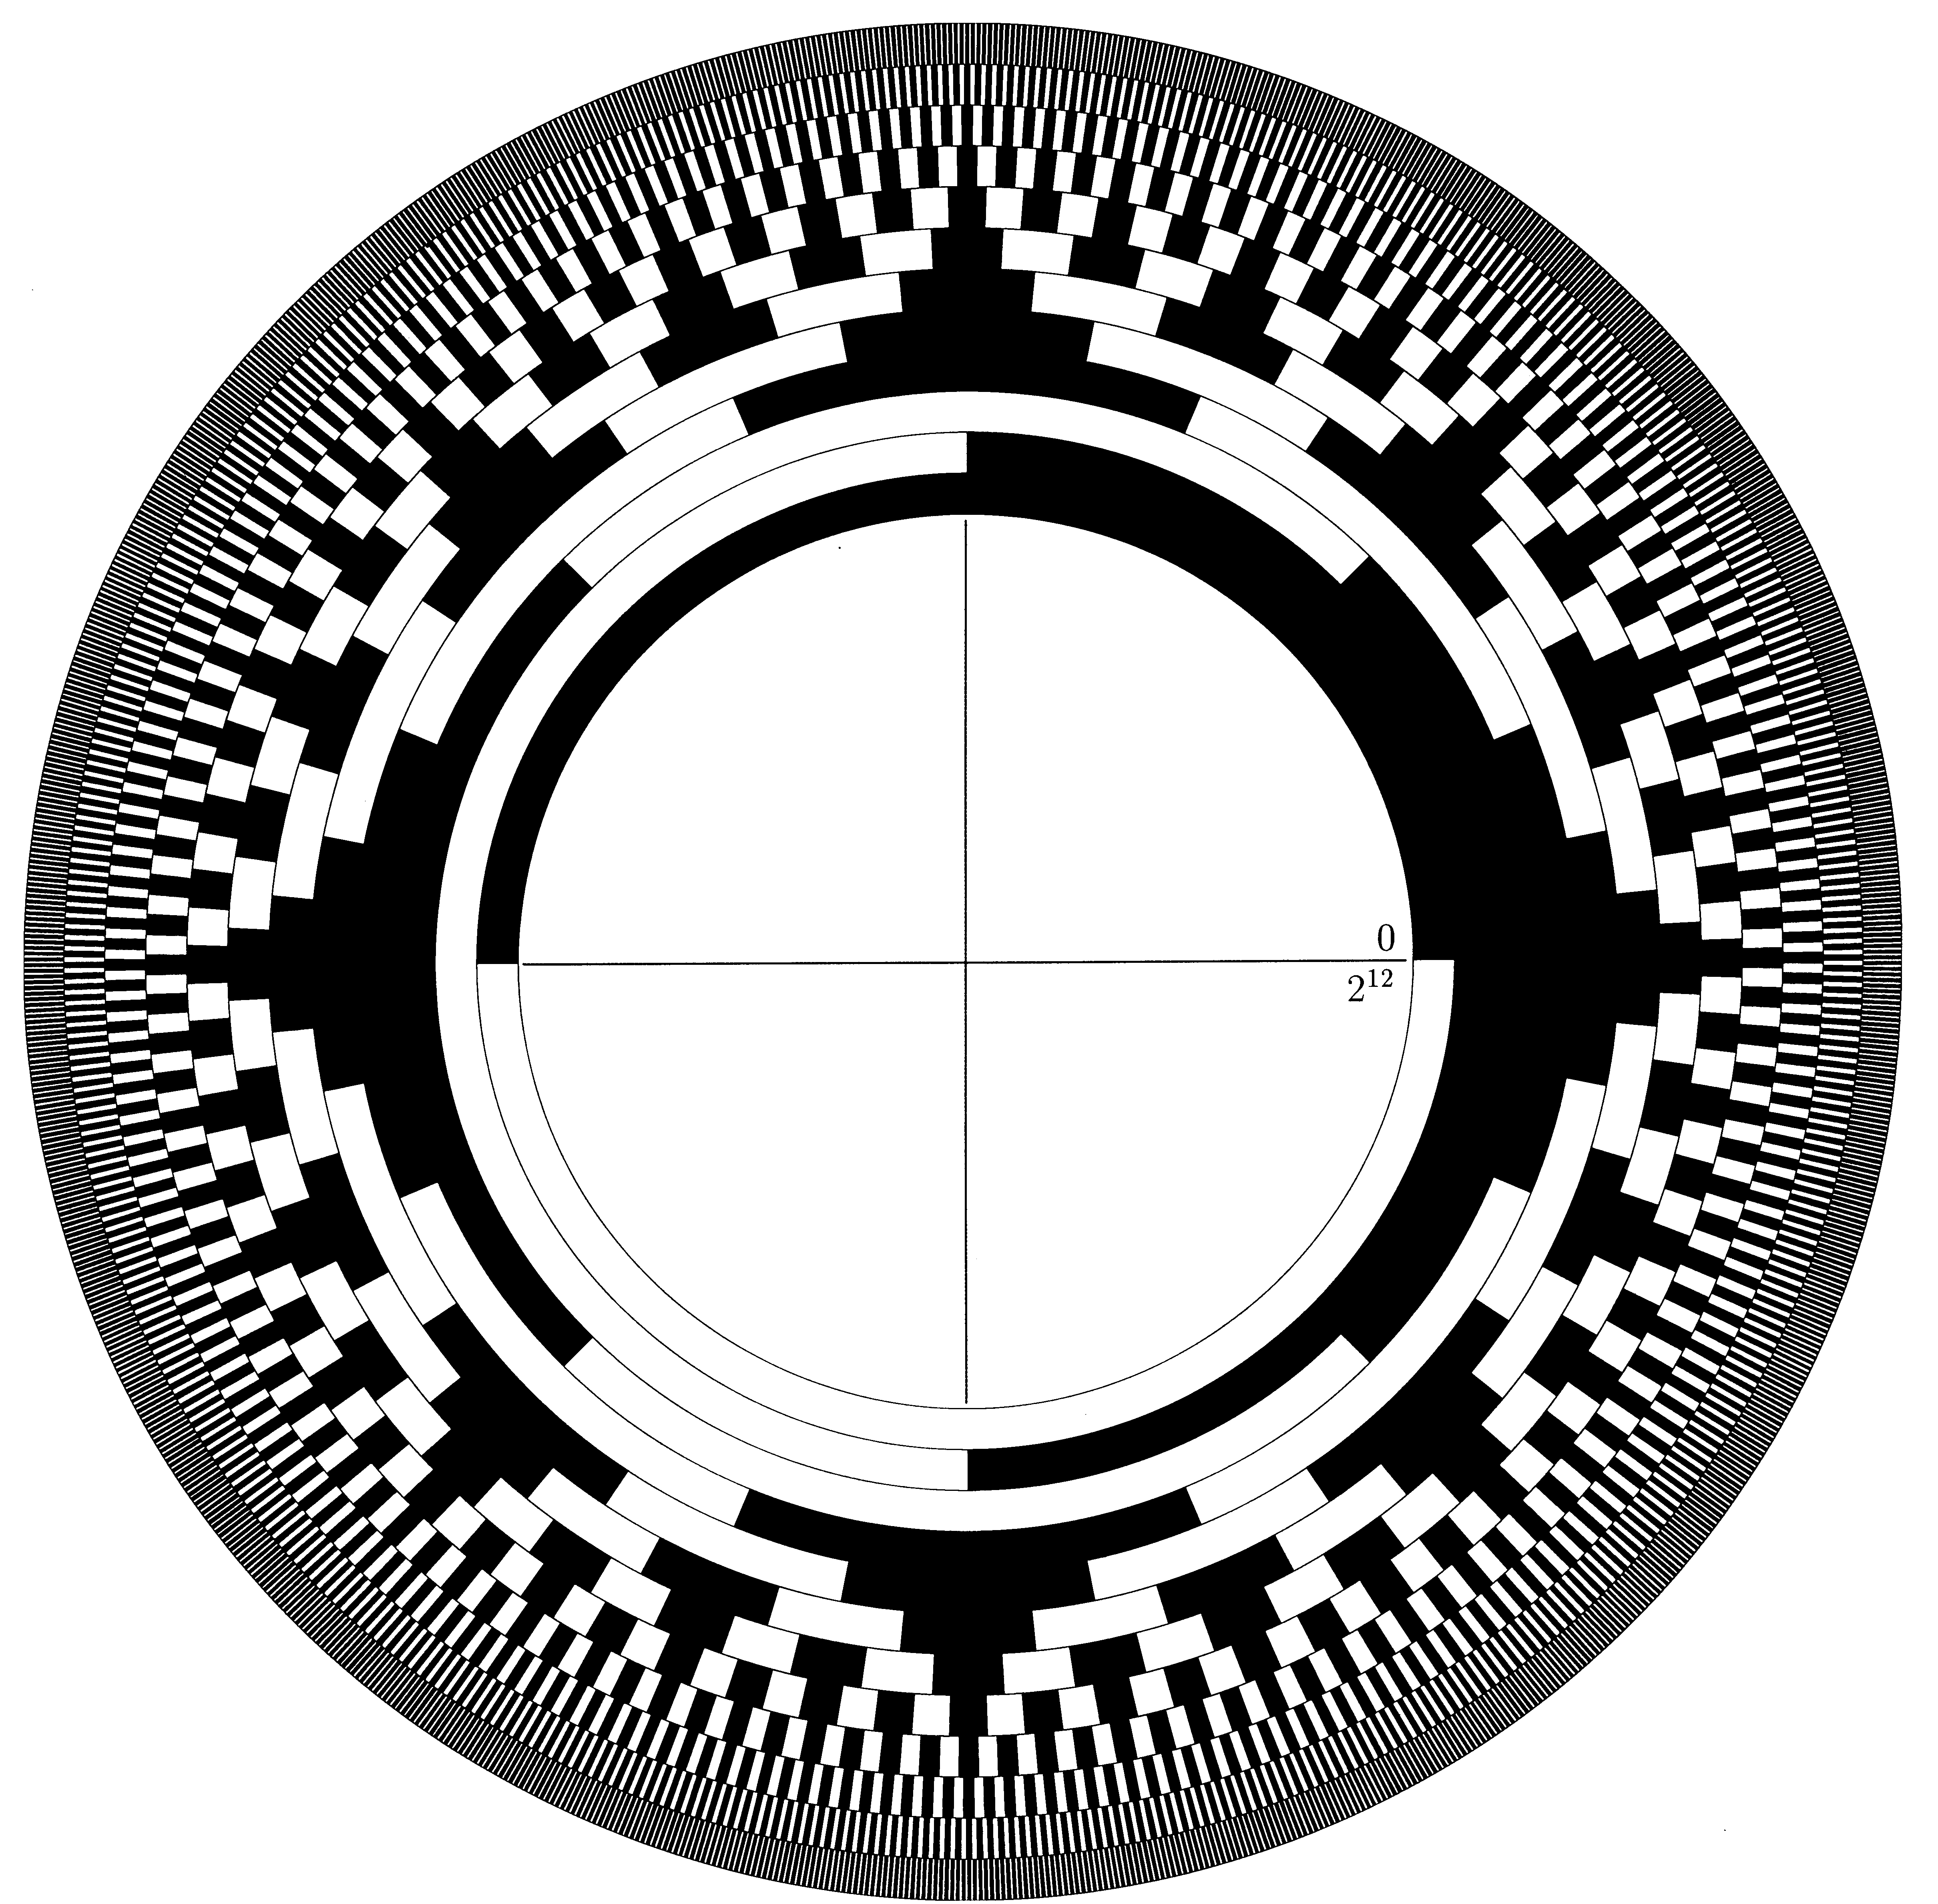
\includegraphics[width=\textwidth]{winkelcodescheibe.png}
	\caption{Die benutzte Winkelcodescheibe -- (4) in \ref{img:pererpen}}
	\label{img:wicosch}
\end{figure}
Die Codescheibe kann den Auslenkwinkel $x$ mit einer Auflösung von bis zu zwölf Bits darstellen. Da für die volle Auflösung eine aufwändige Kalibrierung der Auflichtschranke nötig ist, werden die vier Least-Significant-Bits nicht ausgewertet und es verbleibt eine Auflösung von acht Bits, beziehungsweise $\Delta x=\frac{\unit[360]{\degree}}{2^8}\approx\unit[1,4]{\degree}$ oder $\Delta x=\frac{\unit[2\,\pi]{rad}}{2^8}\approx\unit[2,45\tenpo{-2}]{rad}$. Die Abtastrate beträgt $f\ix{S}=\unit[(200\pm4\tenpo{-4})]{Hz}$, was einer Abtastperiode von $T\ix{S}=\unit[(5\pm1\tenpo{-4})]{ms}$ entspricht. Die Winkelgeschwindigkeit $y$ wird von der Elektronik automatisch aus zwei Auslenkwinkeln im Abstand von 32 Abtastperioden berechnet: $y(t)\approx\frac{x(t)-x(t-32\cdot T\ix{S})}{32\cdot T\ix{S}}$.\\
Ausgegeben werden Spannungen, die um einen zu den Messwerten $x$ und $y$ proportionalen Term verschoben sind:
\begin{align}
U_x(t)=U\ix{max}\cdot\left(\frac{1}{2}+\frac{x(t)}{2\,\pi}\right)\hspace{2em}\text{bzw.}\hspace{2em}U_y(t)=U\ix{max}\cdot\left(\frac{1}{2}+\frac{y(t)\cdot 32\cdot T\ix{S}}{2\,\pi}\right)
\end{align}
Hierbei ist $U\ix{max}=\unit[3,06\,(1)]{V}$ die maximale Ausgabespannung. Es wird ersichtlich, dass $x$ im Intervall $\left[-\pi;\pi\right)$ und $y$ im Intervall $\left[\frac{-\pi}{32\cdot T\ix{S}};\frac{\pi}{32\cdot T\ix{S}}\right)$ gemessen werden. Die Grenzen des Intervalls für den Auslenkwinkel sind offensichtlich, die Grenzen des Intervalls für die Winkelgeschwindigkeit wurden aus der Überlegung heraus gewählt, dass sicher nicht mehr als $\frac{\nicefrac{1}{2}}{32\cdot T\ix{S}}=3,125$ Vollkreise pro Sekunde durchlaufen werden. Die Messgenauigkeit der Winkelgeschwindigkeit beträgt ungefähr $\Delta y\approx\unit[1,047]{rad}$. Mithilfe der Lichtschranke und des Zeigers (siehe Kapitel \ref{ch2.1}) lässt sich auch eine stroboskopische Ausgabe der Messungwerte realisieren: Die Spannungen an den Ausgängen werden nur aktualisiert, wenn der Zeiger die Lichtschranke zweimal durchlaufen hat, also die gleiche Phasenlage der Erregung erreicht ist.
\subsection{Die mathematische Beschreibung der Bewegung}
\subsubsection{Die grundlegende Bewegungsgleichung}
Die Newtonsche Bewegungsgleichung des nicht-erregten, ungedämpften physikalischen Pendels wird als bekannt vorausgesetzt:
\begin{align}
J\cdot\frac{\diff^2 x}{\diff t^2}+m\cdot l\cdot g\cdot\sin\left(x\right)=0\label{eq:bew1}
\end{align}
Hierbei ist $J$ das Trägheitsmoment, $m$ die Masse des gesamten Pendelkörpers, $l$ der Abstand von der Drehachse zum Schwerpunkt des Körpers und $g$ die Fallbeschleunigung im erdnahen Gravitationsfeld. Daraus lässt sich die Eigenfrequenz, die Schwingfrequenz bei kleinen Auslenkungen, zu $f\ix{0}=\frac{1}{2\,\pi}\sqrt{\frac{m\,l\,g}{J}}$ berechnen. Diese lässt sich über den Abstand der Hauptschwingmasse von der Drehachse (im Folgenden wird der Abstand zwischen unterer Fläche der Hauptmasse und Drehachse als $l\ix{0}$ bezeichnet) beeinflussen. Dafür wird $J(l\ix{0})$ berechnet: $J$ setzt sich aus dem Trägheitsmoment des Hauptkörpers, des Stabs, der Codescheibe und der Wirbelstrombremse zusammen. Nur Das Trägheitsmoment des Hauptkörpers $J\ix{K}$ ist von $l\ix{0}$ abhängig und berechnet sich mit dem Trägheitsmoment um eine durch den Schwerpunkt verlaufende Achse $J\ix{K0}$ nach dem Steinerschen Satz zu $J\ix{K}(l\ix{0})=J\ix{K0}+ m\ix{K}\cdot\left(l\ix{0}-\frac{h\ix{K}}{2}\right)^2$, mit $h\ix{K}$ der Höhe und $m\ix{K}$ der Masse des Hauptpendelkörpers. Ist nun das Gesamtträgheitsmoment bei einer festen Länge (zum Beispiel der Länge des Stabs $L\ix{0}$) bekannt, berechnet sich $J(l\ix{0})$ zu:
\begin{align}
	J(l\ix{0})&=J(L\ix{0})+m\ix{K}\cdot\left(\left(l\ix{0}-\frac{h\ix{K}}{2}\right)^2-\left(L\ix{0}-\frac{h\ix{K}}{2}\right)^2\right)\nonumber\\
	&=J(L\ix{0})-m\ix{K}\cdot\left(L\ix{0}^2-l\ix{0}^2-h\ix{K}\cdot\left(L\ix{0}-l\ix{0}\right)\right)
\end{align}
Für den Abstand des Pendelschwerpunkts von der Drehachse $l$ wird noch die Masse des Stabs $m\ix{S}$ und die Schwerpunktslage des Stabs $l\ix{S}$ benötigt. Damit ergibt sich:
\begin{align}
	l(l\ix{0})=\frac{m\ix{S}}{m}\cdot l\ix{S}+\frac{m\ix{K}}{m}\cdot\left(l\ix{0}-\frac{h\ix{K}}{2}\right)
\end{align}
Die Werte $J(L\ix{0})=\unit[34,3(4)]{g\,m^2}$, $L\ix{0}=\unit[400,0(5)]{m}$, $m\ix{K}=\unit[201,93(5)]{g}$, $h\ix{K}=\unit[37,8(1)]{mm}$, $m\ix{S}=\unit[53,87(5)]{g}$, $l\ix{S}=\unit[209(1)]{mm}$, sowie ein praktisches Diagramm zum Ablesen der Eigenfrequenz $f\ix{0}(l\ix{0})$ wurden freundlicherweise in der Versuchsanleitung bereitgestellt.
\subsubsection{Die parametrische Erregung}
Zusätzlich zur Erdbeschleunigung wird das Pendel durch die Auf- und Abbewegung nach oben und unten beschleunigt. Da die Höhe der Drehachse mit der Erregerphase (o.B.d.A. befinde sich der Hebelarm zu $t=0$ am unteren Totpunkt) verändert wird, $h(t)=h\ix{0}-a\cdot\cos\left(\omega\cdot t\right)$, ergibt sich eine Modulation des Parameters $g$ in Gleichung (\ref{eq:bew1}) um $\frac{\diff^2 h}{\diff t^2}=a\cdot\omega^2\cdot\cos\left(\omega\cdot t\right)$ mit der Amplitude $a$ und der Kreisfrequenz $\omega$ der Erregung. Da die Beschleunigung am unteren Totpunkt in die gleiche Richtung wie die Fallbeschleunigung zeigt, wird diese einfach zu $g$ hinzu addiert:
\begin{align}
J\cdot\frac{\diff^2 x}{\diff t^2}+m\cdot l\cdot \left(g+a\cdot\omega^2\cdot\cos\left(\omega\cdot t\right)\right)\cdot\sin\left(x\right)=0\label{eq:bew2}
\end{align}
\subsubsection{Die Dämpfung}
Gleichung (\ref{eq:bew2}) bildet natürlich noch kein reales System ab -- in der Praxis dissipiert immer Energie aus dem System in die Umgebung. Dies geschieht zum einen über die, nicht beeinflussbare, Reibung und zum anderen in unserem Versuchsaufbau über die Bremswirkung der Wirbelstrombremse. Der Einfluss der Reibung hängt näherungsweise nur von der Bewegungsrichtung des Pendels ab und wird mit der experimentell bestimmten Konstante $b\ix{0}=\unit[0,027(3)]{N\,m}$ bewertet. Die Bremswirkung der Wirbelstrombremse hängt von der Stromstärke ab und der Einfluss dieser Bremswirkung auf das System ist proportional zur Geschwindigkeit der Pendelbewegung. Der Proportionalitätsfaktor wird bis zur quadratischen Ordnung genähert durch $b\ix{1}\approx\unit[\left(0,01+0,398\cdot\left(\frac{I}{\unit{A}}\right)+0,392\cdot\left(\frac{I}{\unit{A}}\right)^2\right)]{\frac{N\,m\,s}{2\,\pi}}$. Diese Drehmomente wirken der Bewegung entgegen, also werden sie zur linken Seite von Gleichung (\ref{eq:bew2}) hinzu addiert:
\begin{align}
J\cdot\frac{\diff^2 x}{\diff t^2}+b\ix{0}\cdot\signum\left(\frac{\diff x}{\diff t}\right)+b\ix{1}\cdot\frac{\diff x}{\diff t}+m\cdot l\cdot \left(g+a\cdot\omega^2\cdot\cos\left(\omega\cdot t\right)\right)\cdot\sin\left(x\right)=0\label{eq:bew3}
\end{align}
Zur Vereinfachung dieser Gleichung werden nun die dimensionslose Zeitvariable $\tau=2\cdot\pi\cdot f\ix{0}\cdot t$ und die dimensionslosen Parameter $\Omega=\frac{\omega}{2\cdot\pi\cdot f\ix{0}}$, $\beta\ix{0}=\frac{b\ix{0}}{J\cdot\left(2\cdot\pi\cdot f\ix{0}\right)^2}$,  $\beta\ix{1}=\frac{b\ix{1}}{J\cdot2\cdot\pi\cdot f\ix{0}}$, $\alpha=\frac{\omega^2}{g}\cdot a$ eingeführt. Nach einer Division der Gleichung (\ref{eq:bew3}) durch $J\cdot\left(2\cdot\pi\cdot f\ix{0}\right)^2=m\cdot l\cdot g$ ergibt sich nun die normierte Bewegungsgleichung
\begin{align}
	\ddot{x}+\beta\ix{0}\cdot\signum(\dot{x})+\beta\ix{1}\cdot \dot{x}+\left(1+\alpha\cdot\cos\left(\Omega\cdot\tau\right)\cdot\sin\left(x\right)\right)=0\label{eq:bew4}
\end{align}
\subsection{Die weiterführende Betrachtung}
\subsubsection{Die Bewegungsgleichung und ihr Definitionsbereich}
Gleichung (\ref{eq:bew4}) ist eine hochgradig nichtlineare Differentialgleichung zweiter Ordnung. Durch die Terme $\signum\left(\dot{x}\right)$ und $\cos\left(\Omega\cdot\tau\right)\cdot\sin\left(x\right)$ wird die Lösung erschwert, beziehungsweise im Bereich der elementaren Funktionen unmöglich gemacht. Durch Näherungsverfahren (zum Beispiel nach \textsc{Euler} oder \textsc{Runge}-\textsc{Kutta}) lassen sich jedoch für beliebige Parametersätze und Anfangsbedingungen Aussagen über die Zukunft und die Vergangenheit des Systems machen.\\
Die Anfangsbedingungen bilden ein 3-Tupel $(x\ix{0},y\ix{0},\tau\ix{0})$ und stammen vorerst aus dem $\mathbb{R}^3$. Da die Auslenkung $x$ jedoch Winkel in einem Kreis darstellt, hat ihr Definitionsbereich nur eine Breite von $2\,\pi$. In Kapitel \ref{ch2.2} wird bereits angedeutet, dass dieser Definitionsbereich das halboffene Intervall $\left[-\pi;\pi\right)$ ist. Die Winkelgeschwindigkeit $y$ dagegen kann beliebig groß werden, die Einschränkung in Kapitel \ref{ch2.2} gilt nur für den Messbereich. Da auch $\tau$ nur im Argument einer Winkelfunktion vorkommt, nämlich multipliziert mit der normierten Kreisfrequenz $\Omega$, hat auch der Wertebereich dieser Variable eine endliche Breite. Zur Vereinfachung ersetzen wir die normierte Zeit $\tau$ durch die Phasenlage der Erregung $\Omega\cdot\tau=\omega\cdot t\in\left[0;2\,\pi\right)$. Dadurch sind die Anfangsbedingungen $(x\ix{0},y\ix{0},\omega\cdot t\ix{0})\in\left[-\pi;\pi\right)\times\mathbb{R}\times\left[0;2\,\pi\right)=\mathbb{T}\times\mathbb{R}\times\mathbb{T}$, wobei $\mathbb{T}$ für "`Torus"' steht und den Kreis darstellt. Jeder Punkt in diesem dreidimensionalen Raum legt die Trajektorie des Systems eindeutig fest.
\subsubsection{Bewegungsregime und Bifurkationen}
Je nach Anfangsbedingungen und Parameterwahl fällt die Trajektorie asymptotisch in eines von drei sogenannten Bewegungsregimen: Rotation, Libration oder Chaos. Das Rotationsregime zeichnet sich dadurch aus, dass das Pendel sich nur in eine Richtung bewegt, die Winkelgeschwindigkeit also immer das gleiche Vorzeichen hat. Bei der Libration bewegt sich die Auslenkung immer zwischen zwei Grenzen, das Pendel schwingt also hin und her. Chaotischen Bewegungen fehlt jegliche Periodizität.\\
Hat sich das System in ein periodisches Regime eingeschwungen, führen kleine Veränderungen in einzelnen Kontrollparametern zunächst nur zu geringfügigen Verschiebungen der Phasenbahn und irgendwann stellen sich qualitative Veränderungen der Bahn ein -- im zeitlich kontinuierlichen $(x;y)$ Phasenbild spaltet sie sich auf, im stroboskopischen Phasendiagramm treten doppelt so viele Punkte auf. Dies deutet darauf hin, dass die periodische Bewegung nunmehr nicht nur eine, sondern zwei Erregerperioden braucht, um in den Ausgangszustand zurückzukehren. Dies nennt man Bifurkation. Weitere Veränderung des gewählten Parameters zieht weitere Bifurkationen nach sich, sodass die Periode nun das Vierfache der Erregerperiode beträgt und so weiter. Die Veränderung des Parameters, die nötig ist, um eine Bifurkation zu bewirken, wird von Mal zu Mal geringer, bis die Bewegung irgendwann jegliche Periodizität verliert (Periode $\infty$) und ins Chaos übergeht.
\section{Messungen}
Zuerst wurden die Frequenzen für Schwingungen beliebiger Größe bei ausgeschalteter Wirbelstrombremse und maximalem Abstand des Pendelgewichts gemessen. Die Ergebnisse sind in \ref{img:freq} dargestellt, zusammen mit einer Näherung, die in der Versuchsanleitung vorgeschlagen wurde. Diese Näherung sollte erst ab einer Auslenkung von $\frac{\pi}{2}$ merkliche Abweichungen von der exakten Lösung aufweisen, was mit unserer Messung sehr gut korreliert. Die Messung der Frequenzen erfolgte durch Vermessen der Zeit zwischen zwei Auslenkungsextrema ($\hat{=}\frac{T}{2}$), die der Auslenkung durch Mittelwertbildung der ausgegebenen Spannungen bei diesen Maxima. Der Fehlerbereich hierfür ist großzügig gewählt, nämlich der halbe Unterschied zwischen den beiden Maxima, zuzüglich einer geschätzten Messunsicherheit des Oszilloskops von $\Delta U\approx\unit[30]{mV}$ bei Philipps Messungen, beziehungsweise $\Delta U\approx\unit[3]{mV}$ bei Toms Messungen. Die Diskrepanz erklärt sich durch die Wahl unterschiedlicher Messbereiche. Die Messunsicherheit der Frequenz (das Oszilloskop bot eine Funktion zum "`direkten"' Messen von Frequenzen) haben wir zu $\Delta f\approx\unit[0,03]{Hz}$ geschätzt. Lediglich im Bereich höherer Auslenkungen kommt es zur Abweichung der Näherung von den Messwerten -- aufgrund des eingeschränkten Gültigkeitsbereichs der Näherung entspricht dies aber völlig den Erwartungen. Ein oberflächlicher Vergleich mit der in der Anleitung gegebenen (aber leider nicht näher spezifizierten) Kurve ergibt sogar in diesem Bereich eine Übereinstimmung.
\begin{figure}[H]
	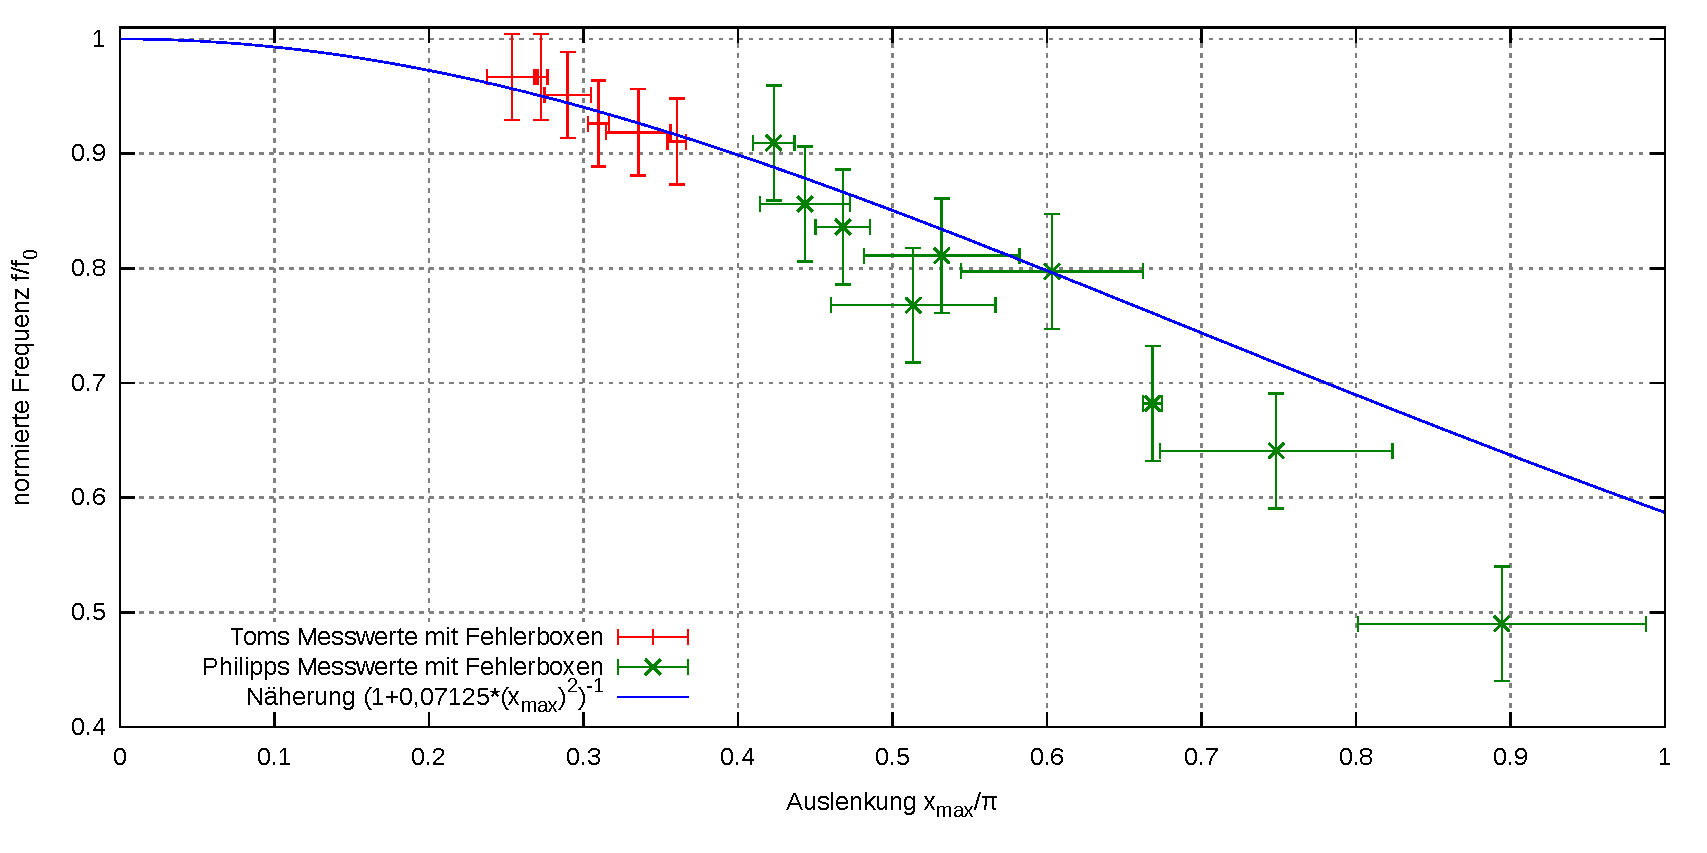
\includegraphics[width=\textwidth]{messwerte/frequenzauslenkung.pdf}
	\caption{Frequenzen der Pendelbewegung bei unterschiedlichen Auslenkungen}
	\label{img:freq}
\end{figure}
Als nächstes wurden Bifurkationen untersucht. Zuerst wurden feste Parameter vorgegeben, das Pendel in ein Rotationsregime getrieben und dann $\beta\ix{1}$ kontinuierlich verändert, bis sich im stroboskopischen Phasenraumbild eine Periodenverdopplung zeigte. Dies wurde für einen ansonsten festen Parametersatz zweimal getan und dann wurde der Abstand des Pendelgewichts von der Drehachse geändert, um $\Omega$ einen neuen Wert zu geben. Nach erfolgreichem Einschwingen im Rotationsregime wurde auch hier wieder $\beta\ix{1}$ kontinuierlich bis zur Periodenverdopplung verändert. Die Ergebnisse zeigt \ref{img:beef}. Unsere Fehlerberechnung stützt sich auf das Gaußsche Fehlerfortpflanzungsgesetz, das wir mit einem CAS auf die funktionalen Zusammenhänge zwischen normierten Parametern und Messgrößen angewendet haben, um letztlich die eingezeichneten Messfehler zu erhalten. Von der Anleitung wurde an dieser Stelle eine Simulation empfohlen, um die Bifurkationsstellen zu verifizieren oder zumindest mit der Simulation zu vergleichen. Da das vorgeschlagene Programm jedoch in unserem Parameterbereich keine auswertbaren Bifurkationsdiagramme geliefert hat, können wir an dieser Stelle leider keinen Vergleich zur Simulation liefern. Da keine Kenntnisse über den Zusammenhang von $\Omega$ und $\beta\ix{1}$ in der Parameterebene bestehen, kann auch kein Rückschluss auf die Qualität der gewonnenen Messwerte gemacht werden. Nichtsdestotrotz beobachteten  wir für die in \ref{img:beef} gezeigten Werte qualitative Bewegungsänderung des Pendels, was den Erwartung aus den Grundlagen gerecht wird.
\begin{figure}[H]
	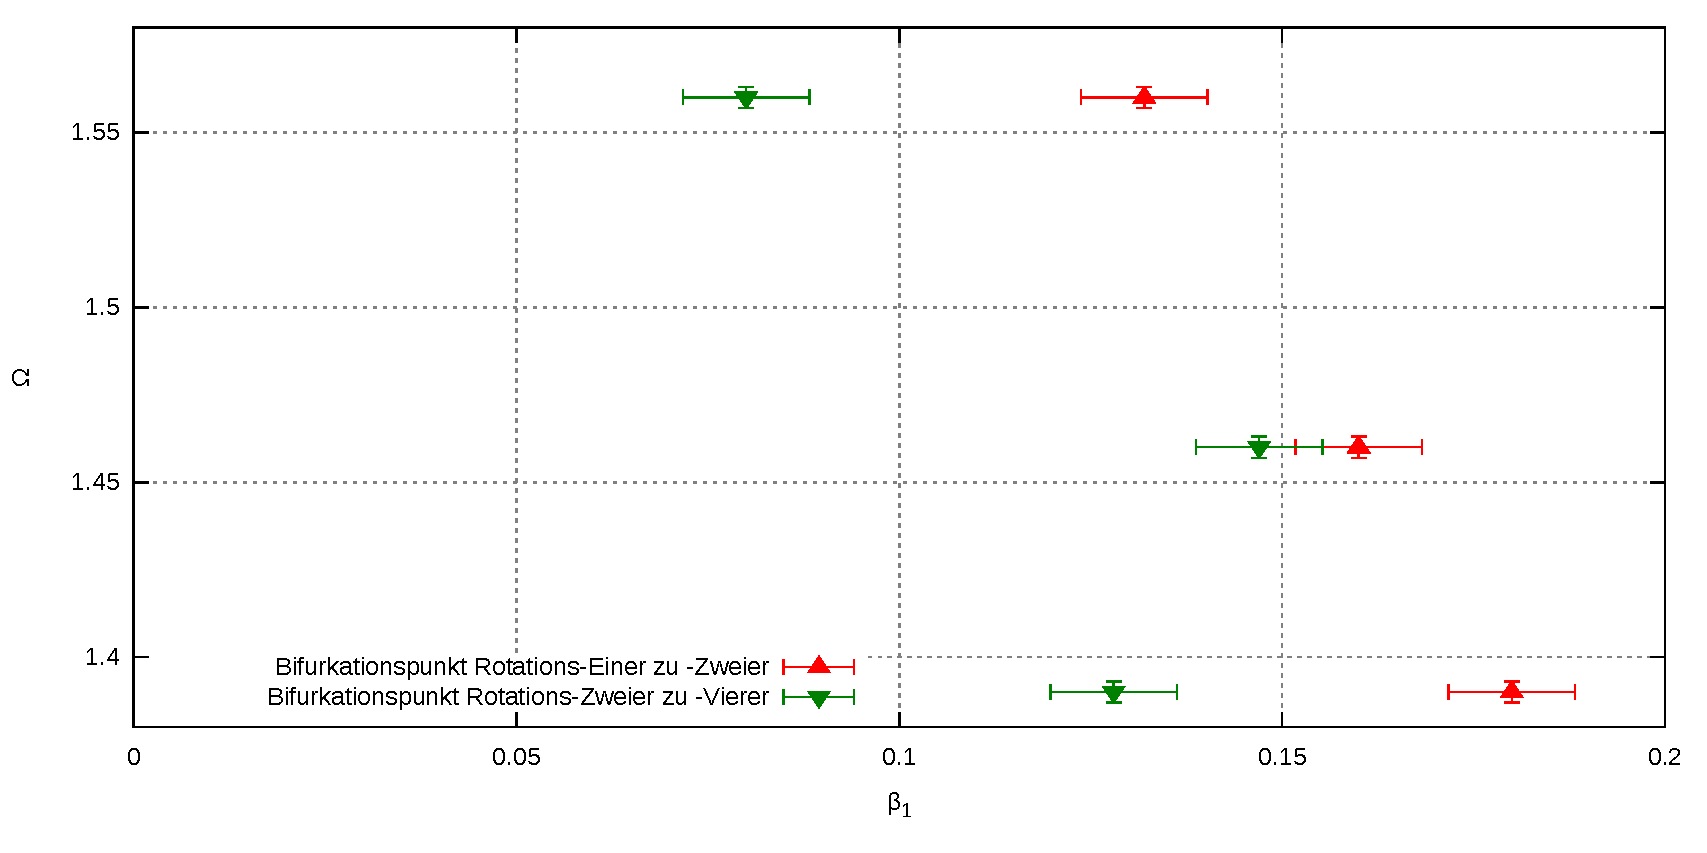
\includegraphics[width=\textwidth]{messwerte/beefurkation.pdf}
	\caption{Punkte in der $(\Omega;\beta\ix{1})$-Parameterebene, bei denen Bifurkationen auftraten}
	\label{img:beef}
\end{figure}
Um Aussagen über den Vorhersagehorizont machen zu können, war es notwendig, zeitsynchron mit der Phase der Erregung die Auslenkung und die Winkelgeschwindigkeit aufzunehmen. Dies war jedoch bei dem gegebenen Versuchsaufbau nicht möglich, weswegen wiederum kein Vergleich zur Simulation angestellt werden konnte. Wir erhielten keine Referenz für die Aussagen über den Vorhersagehorizont. 
\section{Quellen}
\section{Anhang}
Die originalen Messwert-Aufzeichnungen liegen bei.
\end{document}